\section{Alternierung}

\begin{frame}
    \frametitle{Alternierung}
    \framesubtitle{Begriffsklärung}
    Alternierung kann als Verallgemeinerung des Nichtdeterminismus aufgefasst werden, und ist somit ebenfalls ein Konzept, dass in der Praxis kaum umzusetzen ist.
    Während beim Nichtdeterminismus nach einem akzeptierenden Berechnunspfad gesucht wird, können in der Alternierung die Berechnungen quantifiziert werden.
\end{frame}

\subsection{Begriffsklärung}
\begin{frame}
    \frametitle{Alternierung}
    \framesubtitle{Begriffsklärung}
    Die Zustände einer Berechnung einer alternierenden Berechnung sind (neben akzeptierenden und verwerfenden Zuständen) entweder:
    \begin{itemize}
        \item existenziell: Die Berechnung akzeptiert, wenn mind. eine Berechnung akzeptiert
        \item universell: Die Berechnung akzeptiert, wenn alle Berechnungen akzeptieren.
    \end{itemize}
    Bei einem nichtdeterministischen Algorithmus wird lediglich in einem existenziellen Modus operiert,
    sodass wir umgekehrt den Nichtdeterminismus als Spezialfall der Alternierung auffassen können.

\end{frame}


\begin{frame}
    \frametitle{Alternierung}
    \framesubtitle{Alternierender Berechnungsbaum \cite[S.409]{sipser_introduction_2012}}
     \begin{figure}
        \centering
        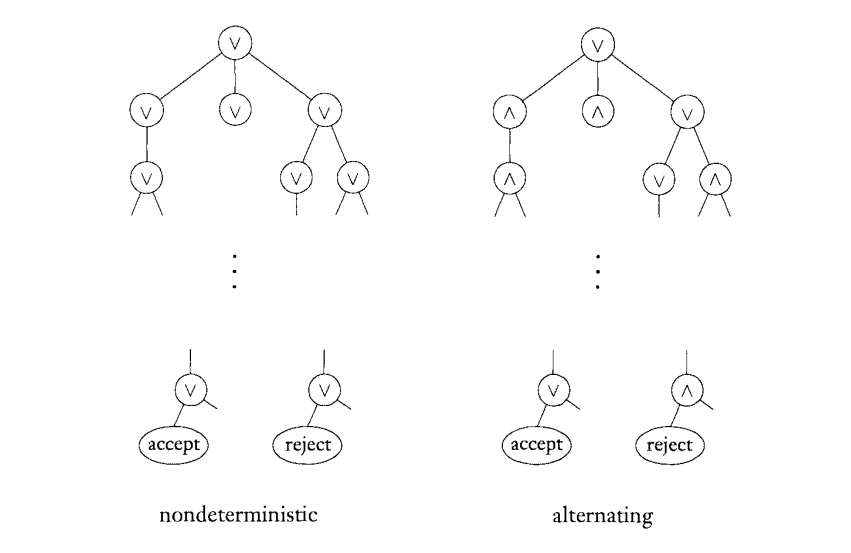
\includegraphics[scale=0.5]{Bilder/Alternierender Berechnugspfad.PNG}
        \label{Alternierende Berechung}
    \end{figure}

\end{frame}

\subsection{Alternierende Turingmaschinen}
\begin{frame}
    \frametitle{Alternierende Turingmaschinen}
    Das Konzept der Alternierung lässt sich auf Turingmaschinen anwenden. 
    Dadurch wird eine neue Klasse von Turingmaschinen definiert, die die Beschränkungen des
    Nichtdeterminismus überwinden.
\end{frame}

\begin{frame}
    \frametitle{Alternierende Turingmaschinen}
    \framesubtitle{Definition}
    \begin{block}{\textbf{Alternierende Turingmaschine}}
        Eine alternierende Turingmaschine ist eine Turingmaschine, die in einem Berechungsschritt in mehrere Zustände übergehen kann,
        und deren Zustände existenziell und universell quantifiziert werden können.
    \end{block}
    Analog zur Betrachtung des Nichtdeterminismus als Spezialfall der Alternierung kann hier eine nichtdeterministische Turingmaschine als Spezialfall einer alternierenden
    Turingmaschine betrachtet werden, die lediglich mit einem existenziellen Zustand ihre Berechnungen durchführt.

\end{frame}

\begin{frame}
    \frametitle{Alternierende Turingmaschinen}
    \framesubtitle{Akzeptanz}
    \begin{block}{\textbf{Akzeptanz einer alternierenden Turingmaschine}}
        Sei $G_{M,x}$ der Konfigurationsgraph einer alternierenden Turingmaschine $M$ auf die Eingabe $x \in \{0, 1\}^*$.
        Dann ist die Akzeptanz von $M$ auf die Eingabe $x$ über folgenden Markierungsalgorithmus definiert:
        \begin{itemize}
            \item Markiere alle Konfiguration terminierend in einem akzeptierenden Zustand $C_{accept}$ mit \texttt{ACCEPT}.
            \item Wenn eine Konfiguration $C$ mit $\exists$ markiert ist, und es eine Kante von $C$ zu $C'$ mit
            Markierung \texttt{ACCEPT} gibt, markiere $C$ mit \texttt{ACCEPT}.
            \item Wenn eine Konfiguration $C$ mit $\forall$ markiert ist, und alle Kanten von $C$ zu
            Konfigurationen $C'$ mit Markierung \texttt{ACCEPT} führen, markiere $C$ mit \texttt{ACCEPT}.
        \end{itemize}
        Die Maschine $M$ akzeptiert genau dann, wenn keine Markierung mehr möglich ist und die Startkonfiguration $C_{start}$ mit \texttt{ACCEPT}
        markiert ist.
    \end{block}

\end{frame}

\begin{frame}
    \frametitle{Alternierende Turingmaschinen}
    \framesubtitle{Alternierende Komplexitätsklassen}
    Alternierende Turingmaschinen werden bezüglich ihrer Zeit- und Platz-Beschränkung ebenso in Komplexitätsklassen unterteilt, wie 
    es für bereits für die ihre deterministischen bzw. nichtdeterministischen Äquivalente bekannt ist.
    \begin{block}{\textbf{Alternierende Komplexitätsklassen}}
        \begin{itemize}
            \item ATIME($f(n)$) ist die Menge aller Sprachen, die von einer $f(n)$-zeitbeschränkten alternierenden Turingmaschine entschieden werden können.
            \item ASPACE($f(n)$) ist die Menge aller Sprachen, die von einer $f(n)$-platzbeschränkten alternierenden Turingmaschine entschieden werden können. 
        \end{itemize}
    \end{block}
    Anhand dieser allgemeinen Definitionen können analog zu DTIME und P, oder NTIME und NP konkrete Komplexitätsklassen definiert werden.
\end{frame}

\begin{frame}
    \frametitle{Alternierende Turingmaschinen}
    \framesubtitle{Alternierende Komplexitätsklassen}
    
    \begin{block}{\textbf{Die Klasse AP}}
        AP = $\bigcup_{c \in \mathbb{N}}$ ATIME($n^c$) \\
        AP ist die Menge aller Sprachen, die von einer polynomiell zeitbeschränkten alternierenden Turingmaschine entschieden werden können.
    \end{block}

    \begin{block}{\textbf{Die Klasse APSPACE}}
        APSPACE = $\bigcup_{c \in \mathbb{N}}$ ASPACE($n^c$) \\
        APSPACE ist die Menge aller Sprachen, die von einer polynomiell platzbeschränkten alternierenden Turingmaschine entschieden werden können.
    \end{block}

\end{frame}


\begin{frame}
    \frametitle{Alternierende Turingmaschinen}
    \framesubtitle{Alternierende Komplexitätsklassen}
    
    Gerade für die Klasse AP ergibt sich dabei ein interessanter Zusammenhang zur Klasse PSPACE:

    \begin{block}{\textbf{Satz}}
        AP $=$ PSPACE
    \end{block}



\end{frame}


\begin{frame}
    \frametitle{Alternierende Turingmaschinen}
    \framesubtitle{AP $=$ PSPACE}
    
    \begin{proof}[Beweis]
        \begin{itemize}
            \item PSPACE $\subseteq$ AP: Simulation einer polynomiell platzbeschränkten TM $M$ durch eine polynomiell zeitbeschränkte ATM $M'$: $M'$ prüft die Erreichbarkeit von zwei Knoten im Konfigurationsgraph von $M$ mit einer angepassten Variante des Satz von Savitch. $M'$ rät existenziell eine Konfiguration zwischen $c_1$ und $c_2$, und prüft dann universell, ob $c_1 c_m$ in höchstens $\frac{k}{2}$ Schritten erreichen kann und selbiges für $c_m$ und $c_2$.
            \item AP $\subseteq$ PSPACE: Simulation einer polynomiell zeitbeschränkten ATM $M$ durch eine polynomiell platzbeschränkten TM $M'$: $M'$ führt eine Tiefensuche im Konfigurationsgraph von $M$ durch und bestimmt die Konfigurationen mit einem akzeptierenden Zustand. $M'$ akzeptiert, wenn ein Pfad rekonstruiert werden kann, sodass der Knoten der Startkonfiguration akzeptiert. 
        \end{itemize}
    \end{proof}
\end{frame}